\section{Model analityczny}

Na diagramie \ref{fig:DiagramKlas} przedstawiony został  diagram klas projektowanego systemu.
Jedną z podjętych decyzji jest wyróżnienie typu wyliczeniowego \textit{TypDokumentu}, który determinuje rodzaj utworzonego dokumentu(WZ lub PZ). Decyzja ta podyktowana była faktem, iż funkcje i atrybuty udostępniane przez oba typy dokumentów są identyczne, a jedyna różnica która pomiędzy nimi istnieje związana jest z kontekstem, w którym występuje dany dokument.

\begin{figure}[!htb]
  \begin{center}
    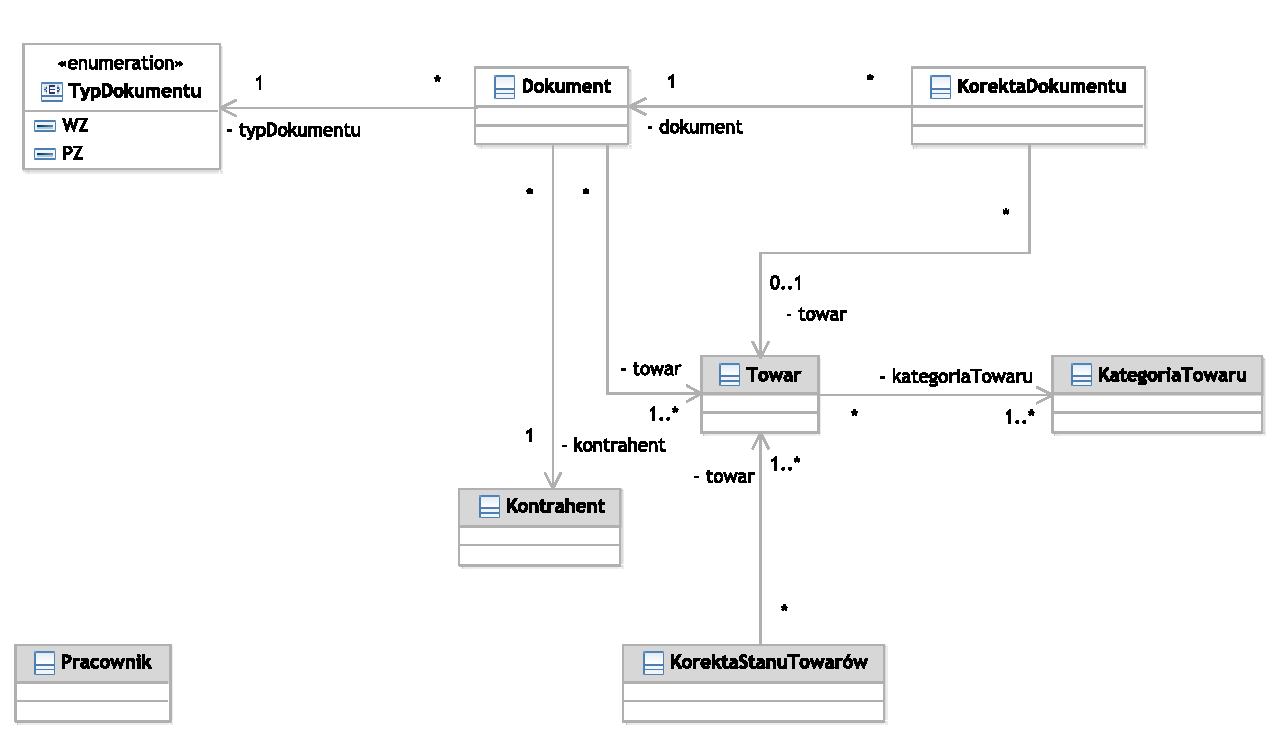
\includegraphics[scale=0.7]{../img/model/diagram_klas.pdf}
  \end{center}
  \caption{Diagram klas}
  \label{fig:DiagramKlas}
\end{figure}
\FloatBarrier

Na kolejnych diagramach przedstawione zostały szczegółowe diagramy klas zaprezentowanych na diagramie \ref{fig:DiagramKlas} uwzględniające atrybuty oraz metody klas. Dane te są zgodne z informacjami przedstawionymi w rozdziale \ref{dziedzina-problemu}

\begin{figure}[!htb]
  \begin{center}
    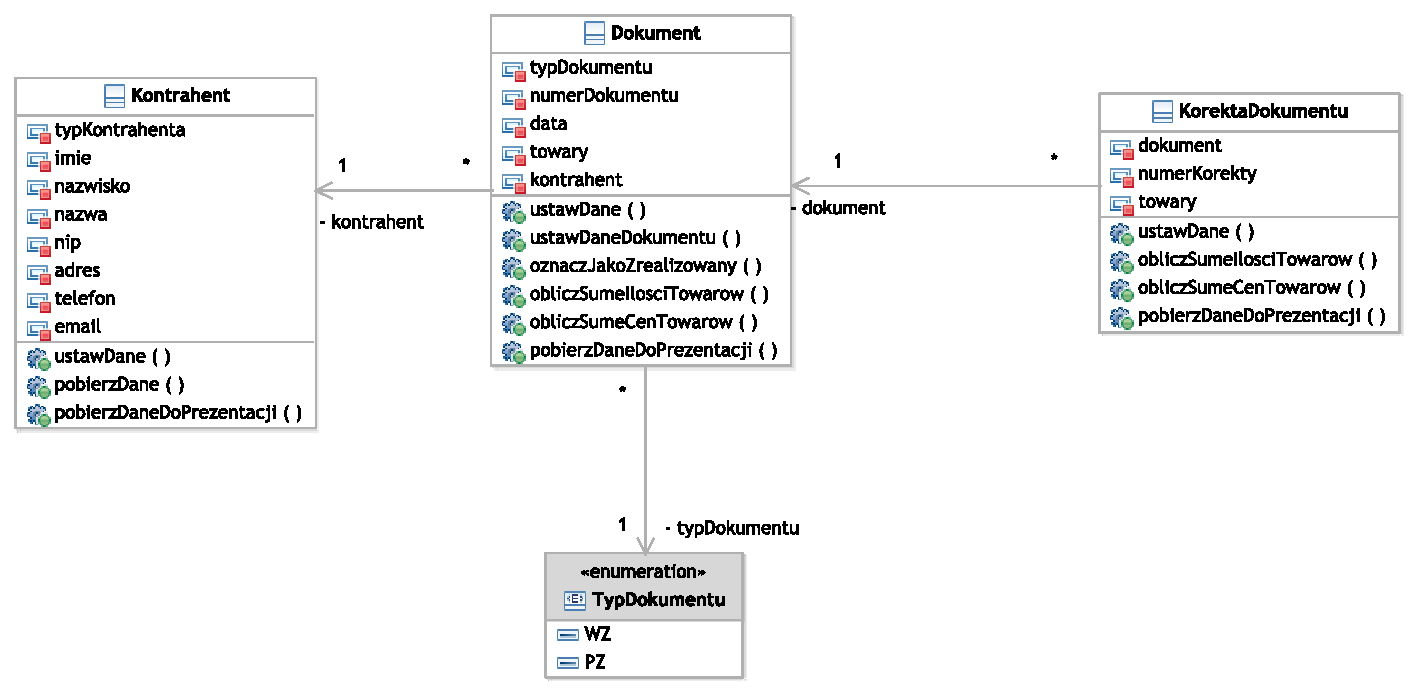
\includegraphics[scale=0.7]{../img/model/diagram_operacja.pdf}
  \end{center}
  \caption{Diagram klas - operacja}
  \label{fig:DiagramKlasOperacja}
\end{figure}
\FloatBarrier

\begin{figure}[!htb]
  \begin{center}
    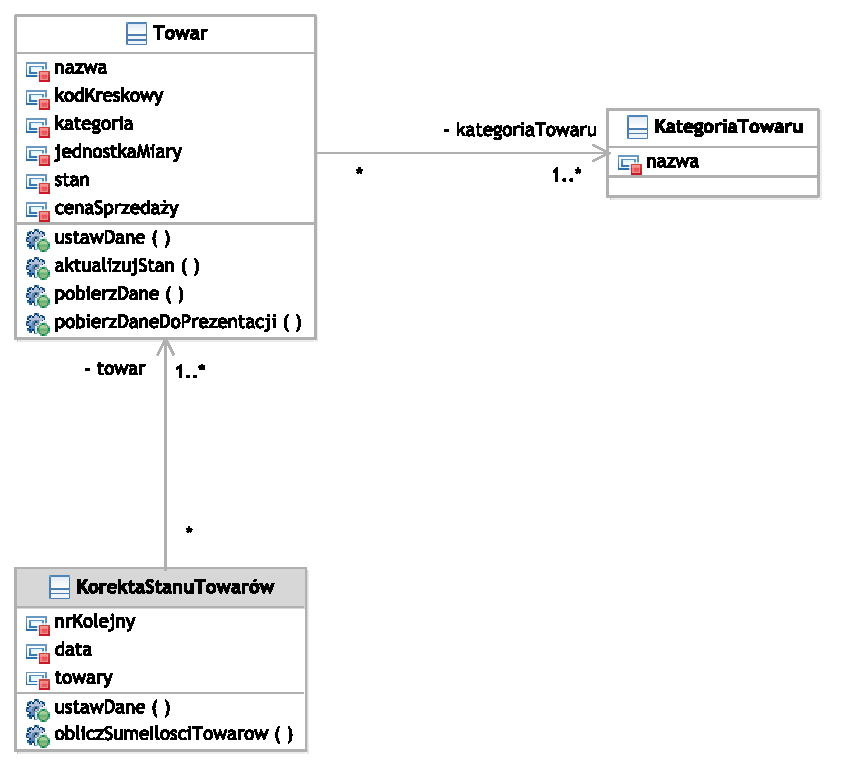
\includegraphics[scale=0.7]{../img/model/diagram_towar.pdf}
  \end{center}
  \caption{Diagram klas - towar}
  \label{fig:DiagramKlasTowar}
\end{figure}
\FloatBarrier

\begin{figure}[!htb]
  \begin{center}
    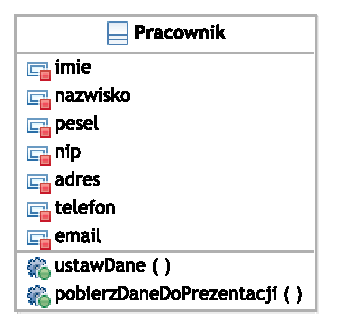
\includegraphics[scale=0.7]{../img/model/diagram_pracownik.pdf}
  \end{center}
  \caption{Diagram klas - pracownik}
  \label{fig:DiagramKlasPracownik}
\end{figure}
\FloatBarrier

Na diagramie \ref{fig:DiagramDAO} przedstawiona została hierarchia klas warstwy dostępu do danych (DAO).

Wprowadzenie hierarchii klas DAO umożliwia stworzenie jednolitego interfejsu pomiędzy źródłem danych i aplikacją. Każda z przedstawionych klas dziedziczy po klasie \textit{AbstractDAO}, która zapewnia dla podstawową implementację operacji na danych.

\begin{figure}[!htb]
  \begin{center}
    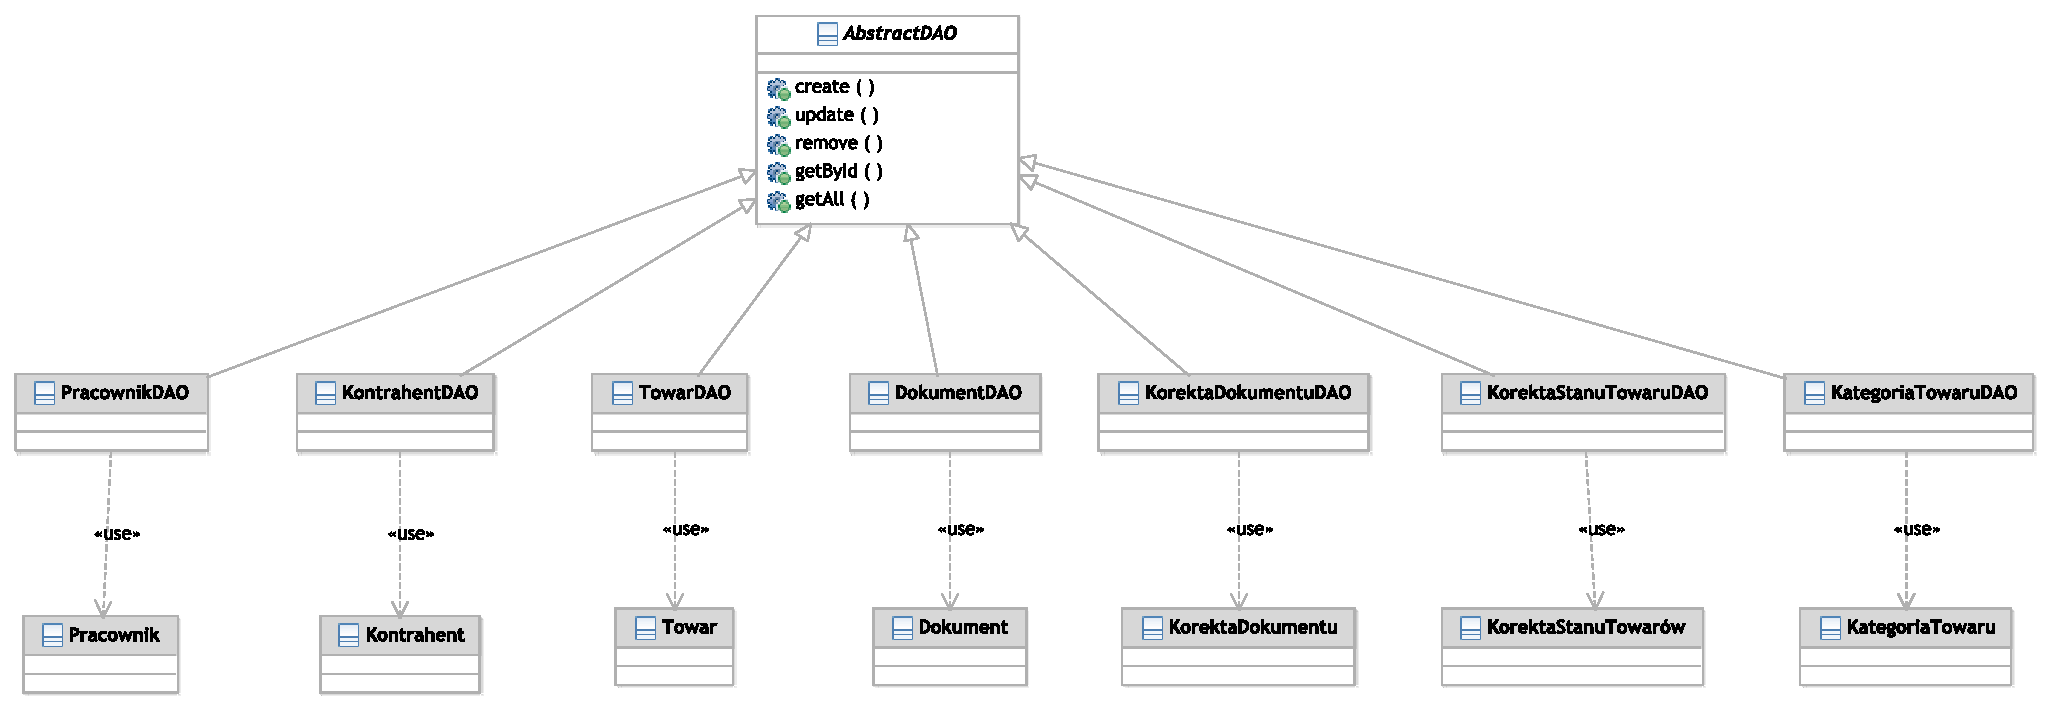
\includegraphics[scale=0.4]{../img/model/diagram_dao.pdf}
  \end{center}
  \caption{Diagram DAO}
  \label{fig:DiagramDAO}
\end{figure}
\FloatBarrier